\chapter{Introdução}
\label{cap:introducao}

\section{Motivação}
Com o crescente uso de scanners ópticos e a laser, modelos 3D (baseados em malha) de alta resolução puderam ser adquiridos com mais facilidade e, dessa forma, utilizados em uma grande variedade de aplicações. Tais scanners, mesmo com resultados fidedignos, falham em produzir modelos completamente sem falhas e ruídos, fazendo com que seu uso seja impraticável em aplicações que necessitam de modelos com alta resolução.
    
\begin{figure}[!ht]
\captionsetup{width=16cm}
\centering
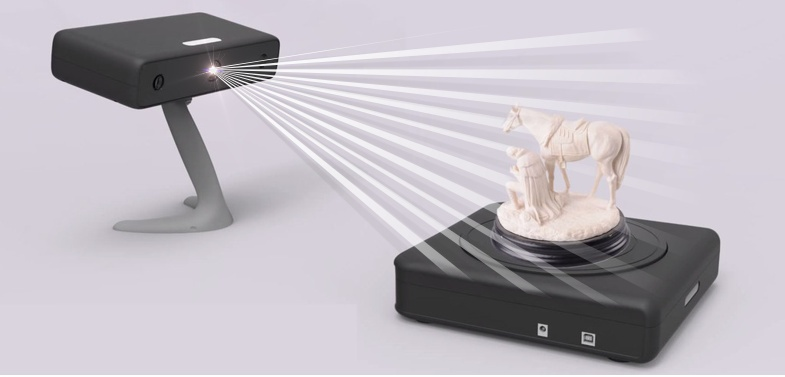
\includegraphics[scale=0.6]{figuras/scan3d.jpg}
\caption{Aquisição de modelo do mundo real por scanner 3D.}
\Fonte{www.3dprintingsystems.com}
\label{fig:scan3d}
\end{figure}

No entanto, otimizar uma malha com ruídos preservando as suas características geométricas não é uma tarefa simples. Efeitos colaterais podem ocorrer, como perda de características e retração ou expansão de volume. Para superar esses desafios, muitas técnicas de otimização de malhas foram propostas nos últimos anos. Essas técnicas fazem parte de uma área chamada Processamento de Geometria, também conhecida como Processamento de Malha, que utiliza conceitos da matemática aplicada, ciência da computação e engenharia para desenvolver algoritmos eficientes para aquisição, reconstrução, análise, manipulação, simulação e transmissão de modelos 3D complexos. Aplicações de algoritmos de processamento de malha cobrem desde áreas de multimídia, entretenimento, CAD, à computação biomédica e científica e engenharia reversa. O nome sugere uma analogia ao processamento de sinais e processamento de imagem. Muitos conceitos, estruturas de dados e algoritmos são diretamente análogos. A técnica de otimização de malha apresentada nesta dissertação se baseia diretamente nos conceitos apresentados em suavização de imagens.

De forma geral, o processamento de geometria trabalha com modelos, geralmente 2D ou 3D, baseados em malha (Figura \ref{fig:mshvsnonmsh}). Processar um modelo envolve três estágios: aquisição, tratamento e finalização. Um modelo pode ser criado por programas de modelagem, representações matemáticas ou scanner. Depois que o modelo é adquirido, ele passa por um processo de otimização, onde todas as falhas e ruídos (Figura \ref{fig:noisymodels}) serão tratados e eliminados. Finalmente, na última fase do processamento, o modelo pode ser utilizado como produto (impressoras 3D) ou em algum outro programa.

\section{Objetivos e Contribuições}

O principal objetivo deste trabalho é apresentar uma técnica de otimização de malhas de filtragem bilateral com um passo de pré-processamento. A técnica proposta visa otimizar, principalmente, malhas que possuem regiões com elementos de baixa qualidade. Entretanto, o método apresentado otimiza com sucesso qualquer tipo de malha com ruído. A técnica foi projetada para atender aos seguintes propósitos:

\begin{itemize}  
\item Detectar regiões com elementos de baixa qualidade que possam atrapalhar a otimização da malha e, então, gerar melhores elementos nessas regiões;
\item Suavizar e remover com sucesso ruídos da malha;
\item Manter, ao máximo, todas as características, detalhes e volume da malha.
\end{itemize}


\begin{figure}[!t]
\captionsetup{width=16cm}
\centering
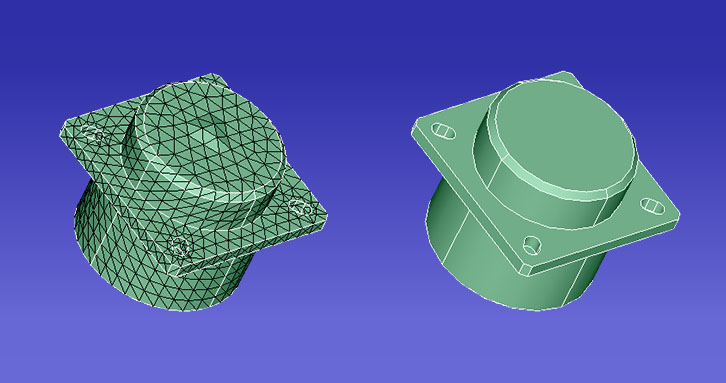
\includegraphics[scale=0.55]{figuras/meshvsnonmesh.jpg}
\caption{Exemplo de modelo 3D baseado em malha e baseado em superfície.}
\Fonte{www.altairhyperworks.com}
\label{fig:mshvsnonmsh}
\end{figure}



\begin{figure}[!t]
\captionsetup{width=13cm}
\centering
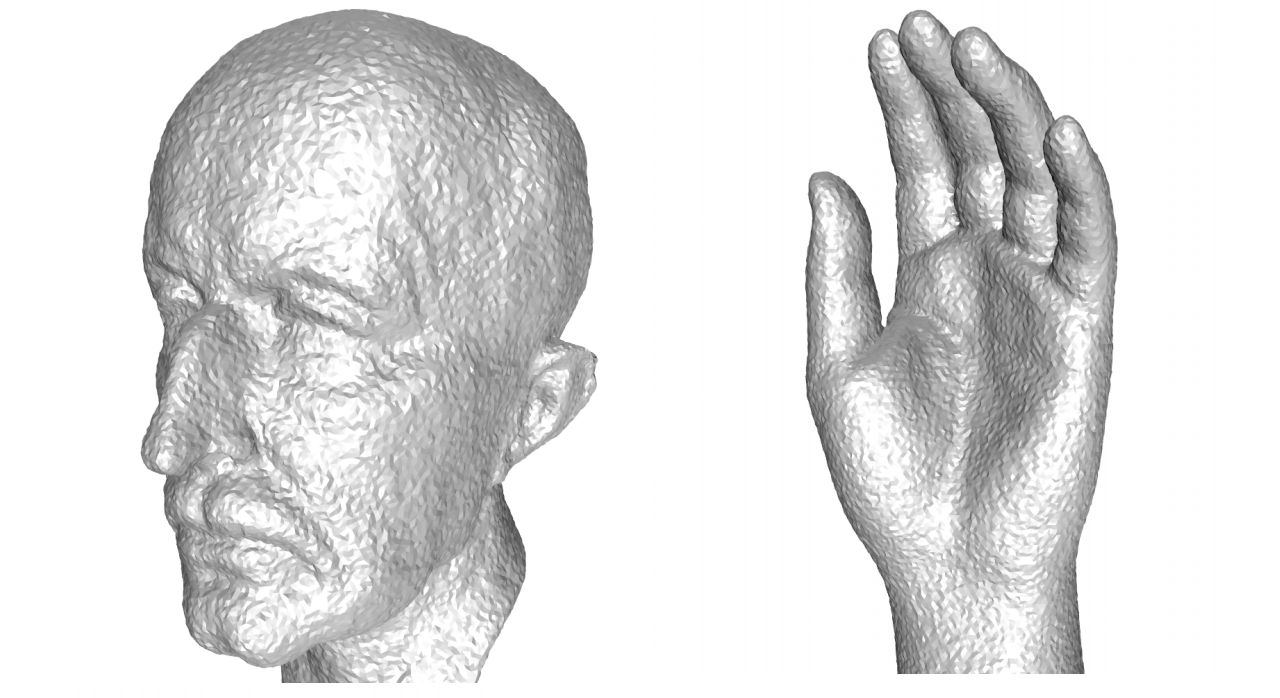
\includegraphics[scale=0.55]{figuras/noisymodels.png}
\caption{Exemplos de modelos 3D com ruídos derivados do processo de aquisição por scanner.}
\Fonte{www.altairhyperworks.com}
\label{fig:noisymodels}
\end{figure}

\section{Organização do Trabalho}
O restante deste trabalho está organizado em quatro capítulos. No Capítulo 2, apresenta-se uma visão geral das técnicas de otimização de malhas com ruídos, dividindo-as em categorias e salientando suas vantagens, desvantagens e propósitos. No Capítulo 3, é apresentada a técnica de otimização de malhas com ruído desenvolvida, detalhando todo o processo e a criação dos modelos de teste. No Capítulo 4, são apresentados os resultados da aplicação da técnica desenvolvida nos modelos de teste criados e em um modelo do mundo real, para demonstrar a sua eficácia. Os resultados obtidos são analisados por métricas para que eles sejam validados com sucesso. Por fim, no Capítulo 5, são expostas as conclusões sobre o trabalho e ideias para futuras melhorias.

